% !TEX TS-program = XeLaTeX
% use the following command:
% all document files must be coded in UTF-8
\documentclass[spanish]{textolivre}
% build HTML with: make4ht -e build.lua -c textolivre.cfg -x -u article "fn-in,svg,pic-align"

\journalname{Texto Livre}
\thevolume{16}
%\thenumber{1} % old template
\theyear{2023}
\receiveddate{\DTMdisplaydate{2023}{6}{6}{-1}} % YYYY MM DD
\accepteddate{\DTMdisplaydate{2023}{7}{12}{-1}}
\publisheddate{\DTMdisplaydate{2023}{8}{22}{-1}}
\corrauthor{Rosa Ana Martín-Vegas}
\articledoi{10.1590/1983-3652.2023.46444}
%\articleid{NNNN} % if the article ID is not the last 5 numbers of its DOI, provide it using \articleid{} commmand 
% list of available sesscions in the journal: articles, dossier, reports, essays, reviews, interviews, editorial
\articlesessionname{articles}
\runningauthor{Martín-Vegas y Seseña-Gómez} 
%\editorname{Leonardo Araújo} % old template
\sectioneditorname{Hugo Heredia Ponce}
\layouteditorname{Thaís Coutinho}

\title{Herramienta tecnológica de evaluación de la comprensión de un texto argumentativo de español lengua materna}
\othertitle{Ferramenta tecnológica para avaliar a compreensão de um texto argumentativo na língua materna espanhola}
\othertitle{Technological tool for reading comprehension assessment of an argumentative text in Spanish as a native language}
% if there is a third language title, add here:
%\othertitle{Artikelvorlage zur Einreichung beim Texto Livre Journal}

\author[1]{Rosa Ana Martín-Vegas~\orcid{0000-0002-7573-9243}\thanks{Email: \href{rosana@usal.es}{rosana@usal.es}}}
\author[1]{Marta Seseña-Gómez~\orcid{0000-0001-6431-1148}\thanks{Email: \href{msesena@usal.es}{msesena@usal.es}}}
\affil[2]{Universidad de Salamanca, Salamanca, España.}

\addbibresource{article.bib}
% use biber instead of bibtex
% $ biber article

% used to create dummy text for the template file
\definecolor{dark-gray}{gray}{0.35} % color used to display dummy texts
\usepackage{lipsum}
\SetLipsumParListSurrounders{\colorlet{oldcolor}{.}\color{dark-gray}}{\color{oldcolor}}

% used here only to provide the XeLaTeX and BibTeX logos
\usepackage{hologo}

% if you use multirows in a table, include the multirow package
\usepackage{multirow}

% provides sidewaysfigure environment
\usepackage{rotating}

% CUSTOM EPIGRAPH - BEGIN 
%%% https://tex.stackexchange.com/questions/193178/specific-epigraph-style
\usepackage{epigraph}
\renewcommand\textflush{flushright}
\makeatletter
\newlength\epitextskip
\pretocmd{\@epitext}{\em}{}{}
\apptocmd{\@epitext}{\em}{}{}
\patchcmd{\epigraph}{\@epitext{#1}\\}{\@epitext{#1}\\[\epitextskip]}{}{}
\makeatother
\setlength\epigraphrule{0pt}
\setlength\epitextskip{0.5ex}
\setlength\epigraphwidth{.7\textwidth}
% CUSTOM EPIGRAPH - END

% LANGUAGE - BEGIN
% ARABIC
% for languages that use special fonts, you must provide the typeface that will be used
% \setotherlanguage{arabic}
% \newfontfamily\arabicfont[Script=Arabic]{Amiri}
% \newfontfamily\arabicfontsf[Script=Arabic]{Amiri}
% \newfontfamily\arabicfonttt[Script=Arabic]{Amiri}
%
% in the article, to add arabic text use: \textlang{arabic}{ ... }
%
% RUSSIAN
% for russian text we also need to define fonts with support for Cyrillic script
% \usepackage{fontspec}
% \setotherlanguage{russian}
% \newfontfamily\cyrillicfont{Times New Roman}
% \newfontfamily\cyrillicfontsf{Times New Roman}[Script=Cyrillic]
% \newfontfamily\cyrillicfonttt{Times New Roman}[Script=Cyrillic]
%
% in the text use \begin{russian} ... \end{russian}
% LANGUAGE - END

% EMOJIS - BEGIN
% to use emoticons in your manuscript
% https://stackoverflow.com/questions/190145/how-to-insert-emoticons-in-latex/57076064
% using font Symbola, which has full support
% the font may be downloaded at:
% https://dn-works.com/ufas/
% add to preamble:
% \newfontfamily\Symbola{Symbola}
% in the text use:
% {\Symbola }
% EMOJIS - END

% LABEL REFERENCE TO DESCRIPTIVE LIST - BEGIN
% reference itens in a descriptive list using their labels instead of numbers
% insert the code below in the preambule:
%\makeatletter
%\let\orgdescriptionlabel\descriptionlabel
%\renewcommand*{\descriptionlabel}[1]{%
%  \let\orglabel\label
%  \let\label\@gobble
%  \phantomsection
%  \edef\@currentlabel{#1\unskip}%
%  \let\label\orglabel
%  \orgdescriptionlabel{#1}%
%}
%\makeatother
%
% in your document, use as illustraded here:
%\begin{description}
%  \item[first\label{itm1}] this is only an example;
%  % ...  add more items
%\end{description}
% LABEL REFERENCE TO DESCRIPTIVE LIST - END


% add line numbers for submission
%\usepackage{lineno}
%\linenumbers
\usepackage{extarrows}


\begin{document}
\maketitle

\begin{polyabstract}
\begin{abstract}
El procedimiento \emph{cloze}, que se emplea habitualmente como herramienta tecnológica para evaluar la comprensión lectora de segundas lenguas, no suele usarse con lenguas maternas. Los motivos que descartan este instrumento con hablantes nativos se basan en que solo detecta el reconocimiento de información y habilidades lingüísticas microestructurales, y no mide la comprensión global ni inferencial del texto. En esta investigación se cuestiona esta idea y, con el fin de dilucidar el valor procedimental, se creó una herramienta de prueba basada en el modelo de exámenes DELE (nivel B2) y se aplicó a estudiantes universitarios españoles ($N=125$) con dos objetivos: 1) medir la comprensión lectora de un texto argumentativo; 2) valorar la comprensión de la coherencia y cohesión discursivas a partir del uso de conectores. La herramienta fue diseñada en Moodle y ejecutada presencialmente. Se midió estadísticamente el índice de acierto y error de cada frase y conector y se aplicaron el test Chi-cuadrado de homogeneidad y el test de Cochran para valorar la significatividad de la confusión entre conectores y nociones argumentales. Los resultados muestran argumentos y conectores más transparentes y patrones de confusión argumental. Se demuestra que esta herramienta basada en el \emph{cloze} mide la comprensión de textos argumentativos en lengua materna y puede ser un instrumento tecnológico replicable.

\keywords{Evaluación \sep Comprensión \sep Lengua materna \sep Test de cloze \sep Argumentación}
\end{abstract}

\begin{portuguese}
\begin{abstract}
 O procedimento \textit{cloze}, comumente utilizado como ferramenta tecnológica para avaliar a compreensão de leitura em segundas línguas, raramente é utilizado com línguas maternas. As razões para descartar esse instrumento com falantes nativos baseiam-se no fato de que ele apenas detecta o reconhecimento de informações e habilidades linguísticas microestruturais, e não mede a compreensão global ou inferencial do texto. Nesta pesquisa, essa ideia é questionada e, para elucidar o valor processual, uma ferramenta de teste baseada no modelo de exame DELE (nível B2) foi criada e aplicada a estudantes universitários espanhóis ($N=125$) com dois objetivos: 1 ) medir a compreensão de leitura de um texto argumentativo; 2) avaliar a compreensão da coerência e coesão discursiva a partir do uso de conectores. A ferramenta foi projetada no Moodle e executada presencialmente. A taxa de acertos e erros de cada sentença e conector foi medida estatisticamente e o teste de homogeneidade Qui-quadrado e o teste de Cochran foram aplicados para avaliar a significância da confusão entre conectores e noções de enredo. Os resultados mostram argumentos e conectores mais transparentes e padrões de confusão de argumentos. Mostra-se que essa ferramenta baseada em \textit{cloze} mede a compreensão de textos argumentativos na língua materna e pode ser um instrumento tecnológico replicável.

    \keywords{Avaliação \sep Compreensão \sep Língua materna \sep Procedimento \textit{cloze} \sep Argumentação}
\end{abstract}
\end{portuguese}

\begin{english}
\begin{abstract}
The cloze procedure, technological tool commonly used to assess reading comprehension in second languages, is not usually used with native speakers. The reasons that rule out this technique with native speakers are based on the fact that it only detects information recognition and microstructural linguistic skills and does not measure global or inferential comprehension of the text. This research questions this idea and, in order to elucidate its procedural value, a tool based on the DELE exam model (level B2) was created and applied to Spanish university students ($N=125$) with two objectives: 1) to measure the reading comprehension of an argumentative text; 2) to assess the comprehension of discourse coherence and cohesion based on the use of linking words. The tool was designed in Moodle and executed in the classroom. The hit and miss rate of each sentence and connector was measured statistically and the Chi-square test of homogeneity and Cochran's test were applied to assess the significance of the confusion between linking words and argumentative notions. The results show more transparent arguments and linking words and patterns of argumental confusion. It is shown that this cloze-based tool measures the comprehension of argumentative texts in the native language and can be a replicable technological instrument.

\keywords{Evaluation \sep Comprehension \sep Mother tongue \sep Cloze procedure \sep Argumentation}
\end{abstract}
\end{english}
% if there is another abstract, insert it here using the same scheme
\end{polyabstract}

\section{Introducción}

Los bajos niveles de comprensión lectora en la lengua materna no solo se constatan de manera recurrente en el ámbito escolar (pruebas del Programa para la Evaluación Internacional de Estudiantes, PISA, realizadas en más de ochenta países al término de la Educación Secundaria Obligatoria), sino que parece que se perpetúan en la edad adulta según los resultados del primer ciclo del Programa para la Evaluación Internacional de las Competencias de los Adultos \cite[los resultados del segundo ciclo se publicarán en 2024]{ministerio2013} y otras investigaciones \cite{gatti2020comprension, duche_comprension_2022}. La dificultad para entender textos densos, identificar argumentos complejos, integrar e interpretar la información… son algunos de los rasgos destacables de estos informes, que reflejan la necesidad de aplicar mejoras educativas dada la asociación evidente entre esta competencia cognitiva y el éxito académico, laboral y social. Consecuentemente, se han desarrollado muchas investigaciones para medir la comprensión lectora de distintos tipos de textos y desde las administraciones educativas se han promovido un sinfín de planes para el fomento lector y el desarrollo de la lectura comprensiva. Pero, a tenor de resultados empíricos actuales, no parecen haber tenido gran efecto en términos generales \cite{robledo_ramon_evaluacion_2019, cabrera-pommiez_evaluacion_2021, canquiz-rincon_planeacion_2021}.

La delimitación conceptual del proceso de comprensión es, en sí misma, muy compleja \cite{sole_competencia_2012, cisneros-estupinan_como_2012, guerra-garcia_variables_2017}, de manera que establecer niveles en función de los múltiples tipos de textos, grupos e individuos sometidos a evaluación resulta un trabajo prolífico en investigaciones y sin resultados concluyentes \cite{scott_what_2018, garcia-martin_metodologias_2020}. La evaluación de la comprensión ha sido la base sobre la que se han sustentado muchos estudios psicopedagógicos para diseñar e implementar de manera experimental estrategias didácticas que les permitieran medir su efectividad. Los instrumentos de evaluación utilizados se basan en test y cuestionarios con preguntas de distinto nivel de profundidad donde los estudiantes identifican información, realizan inferencias conectando ideas, sintetizan ideas globales o secundarias, conectan la información explícita del texto con sus conocimientos previos… (por ejemplo, \textcite{vidal2007tec, garcia2013validacion, felipe_morales_diseno_2018}; o las pruebas de PISA y PIAAC, aplicadas internacionalmente). Estos instrumentos de evaluación son similares en su configuración básica.

En la presente investigación se plantea, como primer aspecto novedoso, la introducción de un modelo instrumental para la evaluación de la comprensión en lengua materna basado en \emph{cloze procedure}, un prototipo tipificado desde hace décadas en la evaluación de segundas lenguas \cite{oller_cloze_1973, sadeghi2021assessing} y, concretamente en el caso del español, fijado en una de las pruebas de comprensión del DELE (Diploma de Español como Lengua Extranjera, Instituto Cervantes). Los beneficios de medición de esta técnica de evaluación aplicada a la comprensión lectora han sido probados en segundas lenguas \cite{jonz_cloze_1991, felicecalzolari2022proceedings}, pero el procedimiento \emph{cloze} no se ha aplicado habitualmente en lengua materna porque se ha considerado, por una parte, que mide habilidades lingüísticas microestructurales que los hablantes nativos dominan y, por otra parte, que no permite medir en su totalidad la comprensión global de un texto \cite{grundin_cloze_1981}. Sin embargo, \textcite{alderson_native_1980} demuestra que los dos grupos de participantes en su muestra, hablantes nativos de inglés y no nativos, tienen un rendimiento similar en las pruebas \emph{cloze} que aplica, por lo que no hay razón para pensar que esta técnica mida solo aspectos básicos de la comprensión literal y no pueda ser válida para hablantes nativos. Y en la misma línea, \textcite{trace_clozing_2020} confirma que la técnica de \emph{cloze} puede medir la comprensión tanto en el nivel de la frase como del discurso completo y tanto en pruebas de lengua materna como de segundas lenguas. De aquí parte el primer objetivo de la presente investigación: demostrar, mediante la aplicación de un modelo instrumental basado en el \emph{cloze procedure}, si es posible medir la comprensión lectora de hablantes nativos de español. 

El segundo objetivo que se plantea, derivado de la aplicación del \emph{cloze procedure} y de la discusión presentada anteriormente, es probar qué información aporta la prueba de evaluación con el fin de poder establecer un modelo instrumental. En este sentido, la investigación se focaliza en las propiedades de coherencia y cohesión que otorgan sentido unitario al texto y permiten comprender, en la terminología clásica vandijkiana, la microestructura (relación de conexión entre proposiciones) y la superestructura (identificación de la organización textual) como estadios previos al desarrollo de inferencias \cite{echevarria2006ensenar}. Así, se ha diseñado una prueba cloze de inserción de oraciones para detectar la comprensión de la coherencia (de la relación lógico-semántica entre las ideas secuenciadas del texto) y de la cohesión (de los indicadores textuales que sirven de nexo entre las oraciones). Son muchos los mecanismos lingüísticos que se usan para cohesionar un texto, pero para la medición de la prueba se han considerado solo los conectores discursivos más trabajados en procesos de composición textual que en comprensión lectora y con un cometido fundamental en el discurso, pues establecen relaciones entre enunciados, orientan el procesamiento de la información y facilitan la comprensión \cite{martinbosque1999}.


\section{Método}

\subsection{Participantes}

El tamaño muestral fue de 125 participantes, todos ellos estudiantes del segundo curso del grado en Maestro de Educación Infantil de la Universidad de Salamanca. Se optó por una muestra homogénea de estudiantes universitarios, con la misma formación académica previa (en todos los casos cursaban su primer grado universitario) y con las características de nivel formativo supuestamente similares que puede tener un grupo de estudiantes del mismo grado y curso.

En relación con las demás variables sociodemográficas que se tuvieron en cuenta, la edad mayoritaria de los encuestados estuvo comprendida entre los 19 y los 21 años (87\%), seguida de los 22 a los 23 años (9,2\%). Los alumnos restantes contaban con más de 24 años (3,8\%) en el momento de la recogida de datos. Como es frecuente en las titulaciones de Ciencias de la Educación y particularmente en el grado de Educación Infantil, la mayoría de las informantes fueron de género femenino (89,6\%).


\subsection{Instrumento}

Se decidió realizar el ejercicio de medición de la comprensión lectora de un texto argumentativo, pues su propia naturaleza los hace más propicios a mostrar más explícitamente los marcadores discursivos que otras tipologías textuales y son, además, junto con los expositivos, los más numerosos en el ámbito académico \cite{martin-macho-harrison_uso_2022}. Se tuvieron en cuenta dos aspectos constructivos importantes en el momento del diseño del texto: \begin{enumerate}
    \item que tuviera una estructura deductiva prototípica descrita como “opinión + argumentos posibles en contra + argumentos con los que nos defendemos + conclusión y cierre” \cite{martinezsanchez2011conectores} y
    \item que, aunque los argumentos defiendan una opinión y, como es consustancial a su tipología, estén destinados a convencer al lector, el texto no tuviera una carga ideológica muy marcada que pudiera sensibilizar a los participantes.
\end{enumerate} 

Adoptamos como modelo de ejercicio una de las pruebas que constituyen la Comprensión Lectora del Diploma de Español como Lengua Extranjera (DELE) de nivel B2 \cite{instituto2014}, pues las características de la propia tarea de medición de capacidades de comprensión lectora basada en la reconstrucción discursiva a nivel cohesivo-semántico sobre un texto argumentativo y el hecho de ser un instrumento de evaluación ampliamente validado a través de las convocatorias anuales que se realizan desde el año 2013 a nivel mundial nos ofrecían la seguridad de estar ante un instrumento fiable. Según el \textcite{instituto2014}, por medio de esta tarea se evalúa la capacidad de reconstruir la estructura de un texto e identificar la relación entre las ideas. Para ello, el candidato debe leer un texto incompleto (de entre 400 y 450 palabras) e identificar, de entre ocho fragmentos posibles, los que corresponden a seis espacios en el texto (se pueden ver ejemplos de exámenes en \url{https://examenes.cervantes.es/es/dele/preparar-prueba}). 

En el proceso de diseño de la prueba se tuvieron en cuenta de forma escrupulosa todas las indicaciones que el Instituto Cervantes marca para que esta tarea sea considerada válida y se incluya en sus exámenes como instrumento de evaluación. En primer lugar, se realizó una búsqueda de un texto adecuado dentro de los ámbitos público, educativo o profesional que, modalmente, correspondiese con un artículo de opinión para, una vez seleccionado, proceder a su adaptación tanto en extensión como en contenidos. Los criterios adicionales que se tuvieron en cuenta para elegir el texto fueron temáticos (se buscaba que los contenidos pudieran resultar interesantes a los grupos que iban a realizar la tarea) y estructurales (el texto elegido debía ser un texto claramente argumentativo en el que se encontrasen varios tipos de conectores o que, al menos, fuese susceptible de poder incluirlos en la adaptación). En este caso no fue necesario adaptar ni el léxico ni las estructuras sintácticas a los contenidos que el Plan Curricular del Instituto Cervantes \cite{instituto2006} marca como prototípicos del nivel B2, pues el ejercicio iba dirigido a hablantes nativos universitarios y se presuponía en ellos un dominio alto de vocabulario y estructuras lingüísticas de carácter culto. La intervención que se realizó al texto elegido estuvo dirigida, principalmente, a reducir la carga político-ideológica y a conseguir un texto de 450 palabras que condensase las ideas principales del texto original por medio de una redacción coherente y bien cohesionada.

El siguiente paso fue determinar cuáles eran los fragmentos que se iban a extraer del texto, teniendo en cuenta que, según las especificaciones de la tarea que se estaba creando, estos debían tener una extensión de entre dieciséis y veinte palabras y formar frases independientes con sentido pleno. Asimismo, se valoró cuál era la relación semántico-pragmática que se establecía entre cada uno de esos fragmentos y su contexto lingüístico previo y posterior, y si esa relación se hacía explícita o no por medio de marcadores discursivos. En los casos en que no aparecía ningún marcador se incluyó el que se consideró más adecuado.

Siguiendo la categorización de marcadores del discurso que ofrece el PCIC en su apartado de Tácticas y estrategias pragmáticas \cite{instituto2006}, en los fragmentos que finalmente se seleccionaron para la prueba, aparecen representados los marcadores discursivos contraargumentativos de introducción de ideas (\emph{no obstante}) y de contraste entre los miembros de la relación (\emph{en cambio}), los aditivos (\emph{más aún}), los recapituladores (\emph{en definitiva}), los rectificativos (\emph{más bien}) y los de refuerzo argumental (\emph{desde luego}).

La última fase de creación de la prueba fue la redacción de los dos distractores. Además de tener una apariencia de validez por su similitud temática con el texto en general y con varios párrafos en particular, se decidió que debían estar introducidos, en la medida de lo posible, por marcadores discursivos de categorías diferentes a las que ya representaban los de los fragmentos extraídos del texto. Teniendo en cuenta la tipología de relaciones semántico-pragmáticas entre ideas esperables en un texto argumentativo, se decidió incluir un conector consecutivo (\emph{así pues}) y un marcador discursivo recapitulador (\emph{en suma}).

El producto de diseño fue un texto con seis espacios intercalados que debían ser completados con seis de las ocho frases que se presentaban como opciones de relleno ordenadas aleatoriamente (\Cref{fig3}). Este texto de prueba se validó mediante un juicio de expertos \cite{escobar2008validez}: tres profesionales con amplia experiencia en la elaboración de la misma prueba de evaluación para el DELE de Cursos Internacionales de la Universidad de Salamanca. A partir de su valoración, se realizaron pequeñas modificaciones relacionadas principalmente con el contenido temático de uno de los distractores. De este modo, se dio por terminado el proceso de creación de la prueba y se procedió a su administración.

\subsection{Procedimiento y plan de análisis de datos}

La prueba se adaptó a la herramienta tecnológica de cuestionario de la plataforma moodle Studium (campus virtual de la Universidad de Salamanca), de uso habitual en la docencia, que permite la visualización del texto con sus huecos y el uso de bloques móviles con las frases para completar que se sitúan en la parte inferior de la pantalla ordenadas para cada participante de manera aleatoria (\Cref{fig3}). La digitalización del texto fue perfecta para el desarrollo de la prueba. El alumno no recibía ningún feedback de acierto o error y podía cambiar las seis opciones elegidas cuantas veces quisiera en el tiempo establecido para el desarrollo del ejercicio, 20 minutos como máximo. La prueba se realizó en el aula de forma síncrona y en presencia de la profesora durante el curso 2022-2023. El tiempo de realización osciló entre los 13 minutos y los 19’15’’.

\begin{figure}[h!]
\centering
\begin{minipage}{1\textwidth}
 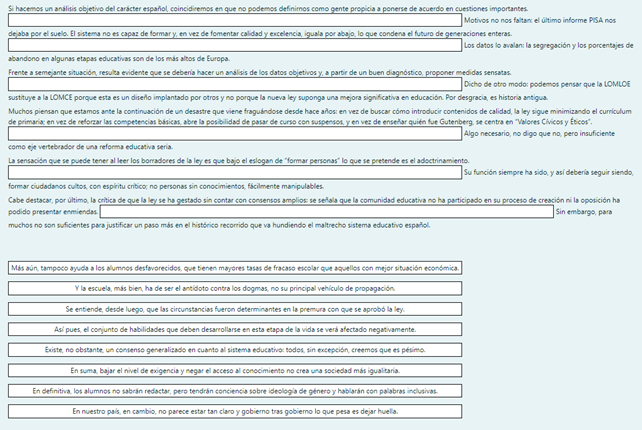
\includegraphics[width=\textwidth]{Fig3.png}
 \caption{Herramienta cloze}
 \source{Elaboración propia}
 \label{fig3}
\end{minipage}
\end{figure}

El análisis estadístico de los resultados de evaluación se llevó a cabo mediante el programa informático SPSS (versión 25). Las técnicas y test aplicados fueron los siguientes: 1) Las variables cualitativas se han descrito mediante tablas de frecuencias, proporciones y porcentajes. 2) La significación de las diferencias entre variables dicotómicas medidas en una misma muestra de sujetos participantes se ha analizado mediante el Test de Cochran. Y 3) se ha aplicado el Test de homogeneidad de Chi-cuadrado para determinar las posibles diferencias entre las opciones de respuesta de variables categóricas. El objetivo ha sido, por una parte, medir estadísticamente el índice de acierto y error de cada frase y su conector, y hacer una valoración de significación de diferencias en los resultados obtenidos entre los seis casos. Por otra parte, mediante el Test de Cochran, se ha valorado qué impacto tiene un determinado uso erróneo de un conector (con su frase) en lugar del conector correcto y, dentro de cada variable correcta, si hay un uso de la frase con el conector erróneo que se utiliza significativamente más que otras frases también incorrectas.

Hemos focalizado los aciertos y errores en el uso de conectores, pese a ser conscientes de que esos conectores forman parte de oraciones donde el conjunto de elementos léxicos constituyen la coherencia discursiva. Pero, en todos los casos, el peso argumentativo decisivo en las opciones correctas para completar el texto dependía del conector discursivo. Por esta razón, como se ha explicado (cf. 2.2), el diseño del instrumento fue un proceso costoso hasta su validación. 


\section{Resultados}

El objetivo de investigación es conocer hasta qué punto este grupo homogéneo de hablantes nativos de español, con una formación académica, son capaces de conectar ideas en textos argumentativos apoyándose en los conectores. Por eso, el análisis de resultados se basa en el uso acertado de conectores y en el uso erróneo (\Cref{tab1}). Por una parte, se ha observado qué conectores (ideas) identifican mejor o peor y, por otra, qué conectores (y nociones argumentales) confunden de manera significativa.


\begin{table}[h!]
\centering
\begin{threeparttable}
\caption{Uso acertado/incorrecto de conectores}
\label{tab1}
\begin{tabular}{llllll}
\toprule
Conector & Errores & Acertantes & \% Acierto & Media & Desv. Est. \\
\midrule
No obstante & 26 & 99 & 79.2\% & 0.79 & 0.41 \\
Más bien & 37 & 88 & 70.4\% & 0.70 & 0.49 \\
Desde luego & 48 & 77 & 61.6\% & 0.62 & 0.50 \\
En definitiva & 49 & 76 & 60.8\% & 0.61 & 0.49 \\
Más aún & 50 & 75 & 60.0\% & 0.60 & 0.46 \\
En cambio & 55 & 70 & 56.0\% & 0.56 & 0.49 \\
\bottomrule
\end{tabular}
\source{Elaboración propia}
\end{threeparttable}
\end{table}


\subsection{Uso correcto de conectores}

La \Cref{fig1} presenta la proporción de acertantes. Se puede apreciar que, sobre un porcentaje medio de aciertos del 65\%, solo dos de ellos, las frases que incluyen los conectores \emph{no obstante} y \emph{más bien}, superan este valor y destacan sobre los demás con más de un 70\% de usos correctos, siendo esta diferencia altamente significativa con $p<.0001$ (Cochran: $Q=26.14$; $\text{P-valor}=.00008$) respecto a las frases con los otros cuatro conectores, que se han usado adecuadamente en una proporción menor y, además, muy similar entre sí (de 56\% al 62\%, sin diferencias significativas entre ellos: $Q=1.26$; $\text{P-valor}=.738$). La diferencia de aciertos entre las frases con los dos conectores con más acertantes (79\% vs. 70\%) está muy cerca de ser significativa también, $p<.10$ ($Q=3.67$; $\text{P-valor}=.056$). Esto parece indicar que la argumentación que liga el conector \textit{no obstante} es la más transparente en la comprensión de forma significativa en nuestra muestra. La contraargumentación y la rectificación de argumentos expresada mediante los conectores \textit{no obstante} y \textit{más bien} se identifican mejor que otras nociones semántico-pragmáticas del texto argumentativo como el refuerzo argumental (\emph{desde luego}), la recapitulación (\emph{en definitiva}), la adición (\emph{aún más}) y la contrastiva (\emph{en cambio}).

\begin{figure}[htbp]
\centering
\begin{minipage}{.8\textwidth}
 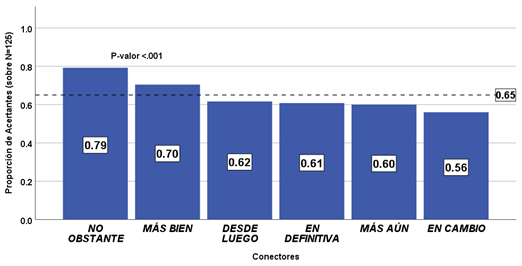
\includegraphics[width=\textwidth]{Fig1.png}
 \caption{Proporción de aciertos en el uso de los conectores}
 \label{fig1}
 \source{Elaboración propia}
\end{minipage}
\end{figure}

Es destacable que las frases que incluyen los dos nexos contraargumentativos (\emph{no obstante} y \emph{en cambio}) se encuentren en los extremos de mayor-menor acierto (\Cref{fig1}). Las diferencias entre ambos conectores no son fáciles de definir \cite{marchante2021}: oposición vs. contraste de argumentos. Sí parece claro, según los resultados de esta investigación, que el argumento de contraste marcado por \textit{en cambio} se ha entendido mucho menos que la noción contraargumentativa de oposición expresada con \textit{no obstante}. Si ligamos estos resultados a la frecuencia de aparición de los conectores en el \emph{Corpus de Referencia del Español Actual} \cite{realacademia} vemos cierta correspondencia (\Cref{tab2}) acorde con el nivel decreciente de aciertos en nuestra prueba; la correlación de resultados solo se altera en el caso de \textit{en cambio}, que es el segundo más usado en CREA después de \textit{no obstante} y el que presenta más fallos en nuestra prueba de comprensión. En cualquier caso, dada la diferencia de uso tan grande entre los dos conectores contraargumentativos (\Cref{tab2}), sí se puede afirmar que la frecuencia de uso de los conectores sea un factor que favorece la comprensión.


\begin{table}[h!]
\centering
\begin{threeparttable}
\caption{Tokens en el \emph{Corpus de Referencia del Español Actual}, CREA}
\label{tab2}
\begin{tabular}{lllllll}
\toprule
Conectores & No obstante & Más bien & Desde luego & En definitiva & Más aún & En cambio \\
\midrule
Tokens & 132.061 & 9.649 & 6.391 & 3.508 & 1.891 & 10.076 \\
\bottomrule
\end{tabular}
\source{Elaboración propia}
\end{threeparttable}
\end{table}

Considerar con estos resultados que hay nociones argumentativas más transparentes que otras y, por tanto, más comprensibles, podría orientar la didáctica del texto al estudio de las relaciones conceptuales con mayor déficit en la comprensión. Según estos datos (\Cref{tab3}), dadas las diferencias significativas en el porcentaje de aciertos de cada conector, deberían trabajarse más aquellas relaciones conceptuales entre argumentos que se comprenden peor.

\begin{table}[h!]
\centering
\begin{threeparttable}
\caption{Comprensión de conectores y nociones semánticas}
\label{tab3}
\begin{tabular}{lllllll}
\toprule
Conectores & No obstante & Más bien & Desde luego & En definitiva & Más aún & En cambio \\
\midrule
\multicolumn{1}{p{1.7cm}}{Nociones semánticas} & oposición & rectificación & refuerzo & recapitulación & adición & contraste \\
& \multicolumn{1}{r}{mejor} & \multicolumn{4}{c}{$\xleftrightarrow{\hspace*{7.75cm}}$} & peor \\
\bottomrule
\end{tabular}
\source{Elaboración propia}
\end{threeparttable}
\end{table}


\subsection{Uso incorrecto de conectores}

En total ha habido 265 errores en el uso de conectores, que da una media de 2.12 por participante, cifra no muy elevada (sobre un máximo de 6) (aunque es reseñable que solo 28 sujetos no cometieron ningún error, 48 tuvieron 3 o más errores y 5 cometieron 6 errores). Esos 265 errores totales, que suponen un 35.3\% sobre el total de las respuestas emitidas ($750=125 \times 6$), se reparten entre los conectores según se indica en la tabla 4. El test de homogeneidad nos indica que hay diferencias altamente significativas ($p<.001$) en cuanto a la frecuencia de uso de cada uno de ellos. Los más usados de forma incorrecta son, sin duda, los dos distractores: \emph{así pues} 57 veces y \emph{en suma} 65 veces, que suponen el 21.5\% y el 24.5\% sobre el total de errores. En los 6 restantes, que se han usado erróneamente entre 18 (\emph{más bien}) y 36 veces (\emph{desde luego}), no se han detectado diferencias significativas ($Chi^2=8.85; P-valor=.117$), es decir, ningún uso erróneo destaca significativamente sobre el resto.


\begin{table}[h!]
\centering
\begin{threeparttable}
\caption{Distribución del uso incorrecto total de los conectores (N=125; 750 respuestas)}
\label{tab4}
\begin{tabular}{llllllllllll}
\toprule
\multirow{2}{*}{} &  & \multicolumn{8}{c}{Conectores} & \multicolumn{2}{>{\raggedright}p{2cm}}{Test Homogeneidad} \\
\cmidrule{3-10}
 & \rotatebox{90}{Nº total} & \rotatebox{90}{No obstante} & \rotatebox{90}{Más bien} & \rotatebox{90}{Desde luego} & \rotatebox{90}{En definitiva} & \rotatebox{90}{Más aún} & \rotatebox{90}{En cambio} & \rotatebox{90}{Así pues} & \rotatebox{90}{En suma} & Valor & P-valor \\
 \midrule
\multicolumn{1}{>{\raggedright}p{1.5cm}}{Nº total de errores} & 265 & 22 & 18 & 36 & 19 & 23 & 25 & 57 & 65 & 69.88 & .0000 \\
\bottomrule
\end{tabular}
\source{Elaboración propia}
\end{threeparttable}
\end{table}

A continuación, se estudió, con el objetivo de determinar si hay un patrón definido de uso, si, para cada uno de los conectores, los errores se distribuyen de forma homogénea o no (\Cref{tab5}). Se ha comprobado que en 5 de los 6 conectores hay usos incorrectos de algún otro conector que son más frecuentes que otros. El único donde no ocurre esto es en \emph{desde luego} ($p>.05$), donde no hay un error que destaque sobre los demás y, por tanto, no se encuentra el patrón buscado. Por su parte, sí aparece en los restantes:

\begin{enumerate}
    \item Donde se debería haber usado \emph{no obstante}, los errores más frecuentes de forma muy significativa ($p<.01$) son \emph{en cambio} y \emph{así pues}.
    \item Donde se debería haber usado \emph{más bien}, los errores más frecuentes con significación estadística ($p<.05$) son \emph{en definitiva} y \emph{así pues}.
    \item Donde se debería haber usado \emph{en definitiva} los errores más frecuentes con significación estadística ($p<.05$) son \emph{en suma}, \emph{así pues} y, en menor medida, \emph{desde luego}.
    \item Donde se debería haber usado \emph{más aún}, los errores más frecuentes de manera muy altamente significativa ($p<.001$) son \emph{en suma} y \emph{así pues}.
    \item Y donde se debería haber usado \emph{en cambio}, el error más frecuente de forma muy significativa ($p<.01$) es \emph{desde luego}, seguido en menor medida de \emph{en suma}.
\end{enumerate}


\begin{table}[h!]
\centering
\begin{threeparttable}
\caption{Distribución del uso incorrecto de cada uno de los conectores}
\label{tab5}
\begin{tabular}{llllllllllll}
\toprule
 &  & \multicolumn{8}{c}{Conectores} &  \multicolumn{2}{>{\raggedright}p{2cm}}{Test Homogeneidad} \\
\cmidrule{3-10} 
 Conector & \rotatebox{90}{Total de errores} & \rotatebox{90}{No obstante} & \rotatebox{90}{Más bien} & \rotatebox{90}{Desde luego} & \rotatebox{90}{En definitiva} & \rotatebox{90}{Más aún} & \rotatebox{90}{En cambio} & \rotatebox{90}{Así pues} & \rotatebox{90}{En suma} &  Valor & P-valor \\
\midrule
No obstante & 26 &  & 3 & 1 & - & 2 & 12 & 7 & 1 & 22.00 & .0007 \\
Más bien & 37 & - &  & 4 & 11 & 3 & 2 & 11 & 6 & 12.78 & .0260 \\
Desde luego & 48 & 12 & 6 &  & 8 & 6 & 5 & 5 & 6 & 5.38 & .5150 \\
En definitiva & 49 & - & - & 10 &  & 3 & 4 & 15 & 17 & 16.20 & .0028 \\
Más aún & 50 & 5 & 3 & 2 & - &  & 2 & 14 & 24 & 47.68 & .0000 \\
En cambio & 55 & 5 & 6 & 19 & - & 9 &  & 5 & 11 & 15.80 & .0075 \\
\bottomrule
\end{tabular}
\source{Elaboración propia}
\end{threeparttable}
\end{table}

Si se interpreta esta confusión en clave argumental, se establecen las siguientes conclusiones:

\begin{enumerate}
    \item\label{conf01} Se confunde la contraargumentación que introduce ideas (\emph{no obstante}) con la contrastiva (\emph{en cambio}) y la consecutiva (\emph{así pues}).
    \item\label{conf02} Se confunde el argumento de rectificación (introducido por \emph{más bien}) con el recapitulador (\emph{en definitiva}) y el que muestra consecuencia (\emph{así pues}).
    \item\label{conf03} Se confunde el argumento que recapitula (\emph{en definitiva}) con el reformulador (\emph{en suma}) y el consecutivo (\emph{así pues}), principalmente.
    \item\label{conf04} Se confunde el argumento de adición (\emph{más aún}), con el reformulador (\emph{en suma}) y el consecutivo (\emph{así pues}).
    \item\label{conf05} Se confunde la contraargumentación contrastiva de ideas (\emph{en cambio}), con el refuerzo argumental (\emph{desde luego}).
\end{enumerate}

La confusión entre los dos nexos contraargumentativos (\ref{conf01}) es previsible, pues los matices semánticos son sutiles. Sin embargo, sí es llamativa la confusión entre una contraargumentación y una consecuencia, pues se trata de argumentaciones opuestas. La confusión (\ref{conf03}) es igualmente en todos sus elementos previsible, pues un argumento de consecuencia puede asociarse a otro anterior como reformulador o recapitulador. Y del mismo modo, la confusión de conectores en (\ref{conf04}) es predecible hasta el punto de que en algunas clasificaciones el reformulador \emph{en suma} se señala como aditivo. Encaja menos dentro de la lógica semántica la confusión de argumentos de (\ref{conf02}) y (\ref{conf05}): rectificar y recapitular ideas son procesos discursivos distintos, igual que contrastar argumentos y reforzarlos.

Los resultados de esta investigación promueven una orientación didáctica de la comprensión textual basada en la conexión semántica y formal entre argumentos. El mal uso de los conectores indica confusión entre las nociones argumentales que unen. Por este motivo, la didáctica debería centrarse en aquellos argumentos dispares que se confunden por falta de comprensión (\Cref{tab6}). Es decir, la medición de la comprensión de un texto argumentativo a través de una prueba como la llevada a cabo en esta investigación conduce a resultados que focalizan el centro de atención didáctico en la conexión de argumentos, pues, a pesar de que todos los hablantes son nativos de español y conocen los conectores, se ha demostrado que no comprenden las relaciones semántico-discursivas que enlazan. 

\begin{table}[h!]
\centering
\begin{threeparttable}
\caption{Confusión de conectores y nociones semánticas}
\label{tab6}
\begin{tabular}{l *{3}{p{3cm}}}
\toprule
Conectores & no obstante vs. así pues & más bien vs. en definitiva & desde luego vs. en cambio \\
\midrule
Nociones semánticas & contraargumentar vs. consecuencia & rectificar vs. recapitular & reforzar vs. contraargumentar \\
\bottomrule
\end{tabular}
\source{Elaboración propia}
\end{threeparttable}
\end{table}

Las confusiones más significativas y no predecibles entre conectores y nociones semánticas (\Cref{tab6}) se corresponden con los mismos niveles de comprensión (\Cref{tab3}). Los tres conectores (\emph{no obstante, más bien} y \emph{desde luego}) y las tres nociones (contraargumentación, rectificación y refuerzo de argumento) que mejor se reconocen según los resultados de esta investigación no se confunden entre ellas de manera significativa (\Cref{tab3}). Son los conectores usados como distractores en la prueba (\emph{así pues} y \emph{en definitiva}) los que producen más errores significativos con todos los conectores excepto con \emph{desde luego}. En este caso, \emph{desde luego} se confunde con todos los conectores sin ningún patrón destacable, pero \emph{en cambio} sí es suplantado en el texto erróneamente por \emph{desde luego} de manera significativa (19 respuestas vs. 5 en dirección inversa). La transparencia del refuerzo argumentativo es mejor en términos generales que la de una contraargumentación contrastiva (\Cref{fig1}, \Cref{tab3}) y apenas hay casos erróneos que usen \textit{en cambio} por \emph{desde luego} (5 usos); sin embargo, la contraargumentación que liga \emph{en cambio} sí está marcada por la confusión con \emph{desde luego} (19 usos). Estos ejemplos merecen una atención especial por la distancia conceptual de los argumentos que conectan, lo que muestra que no es el desconocimiento de los conectores el máximo problema para la comprensión, sino el desconocimiento de los argumentos oracionales.



\section{Discusión y conclusiones}

La comprensión lectora de todo tipo de textos es un tema preocupante en la etapa escolar \cite{martin-ruiz_alisis_2022, caracas_sanchez_evaluacion_2019}. Los resultados obtenidos en las pruebas de competencia lectora según los informes de PISA \cite{ministeriodeeducacion2020} son muy bajos. Además, investigaciones como la presente, llevadas a cabo con estudiantes universitarios, muestran igualmente que los índices bajos de comprensión se extienden a contextos de distintas etapas de la edad adulta \cite{gatti2020comprension, duche_comprension_2022, guerra2022evaluacion}. 

En los últimos años se han realizado estudios metacognitivos que han desarrollado instrumentos para evaluar estrategias de comprensión lectora de textos expositivos \cite{lopez-escribano_predictive_2013, madariagaorbea2010teaching, soriano-ferrer_instruccion_2013} y narrativos \cite{larranaga_evaluacion_2015} que pueden redundar en la didáctica. También se ha estudiado el proceso de comprensión del texto argumentativo, de mayor complejidad estructural, experimentando cómo la escritura de textos es una estrategia que favorece la comprensión \cite{dolz_writing_1995} o no \cite{garate_written_2007}, aplicando el modelo dialogal \cite{alvarez_dificultades_2017} o el enfoque del entorno de aprendizaje constructivista \cite{muhlen_how_2019}, por señalar solo algunos ejemplos significativos de intervenciones diferentes. Los distintos estudios han buscado diagnosticar problemas concretos en la comprensión de este tipo de textos con el objetivo de poder diseñar intervenciones para su mejora. Y se han centrado en la complejidad del proceso de comprensión patente en los textos argumentativos debido a su estructura (exposición de una tesis, relación de argumentos para su defensa y refutación de ideas contrarias, y conclusión a partir del razonamiento lógico derivado de los argumentos precedentes) más que en las propiedades textuales de adecuación, coherencia y cohesión, muy específicas en los textos argumentativos.

El uso de conectores discursivos en los textos argumentativos es muy superior al de otro tipo de textos porque se defienden ideas mediante argumentos con el objetivo, generalmente, de convencer. De este modo, los conectores se usan como elementos de cohesión entre argumentos permitiendo que el razonamiento siga un orden lógico; estos indicadores discursivos dan unidad y sentido global al texto estableciendo relaciones argumentales de oposición, consecuencia, recapitulación etc. Sin embargo, siendo destacables en la cohesión de los textos argumentativos, no se han tenido en cuenta en estudios precedentes como posibles predictores de una deficiente comprensión de los textos. \textcite{martin-macho-harrison_uso_2022} estudian el uso de los conectores de inicio de párrafo en textos argumentativos redactados por hablantes españoles en su lengua materna (L1) y en inglés (L2) con el objetivo de observar una posible transferencia entre lenguas y concluyen que hay una deficiencia general en el uso de conectores que se detecta en el paralelismo en las producciones en ambas lenguas. No ahondan en el tema de la comprensión de los textos (se basan en redacciones de los participantes), pero sí perciben una pobre competencia discursiva basándose en el escaso y poco variado uso de conectores.

En la presente investigación, se ha trabajado la comprensión de textos argumentativos a partir de una herramienta de evaluación \emph{cloze} centrada en los conectores. Hemos trabajado con ocho conectores de distinta tipología: contraargumentativos de introducción de ideas (\emph{no obstante}) y de contraste (\emph{en cambio}), aditivo (\emph{más aún}), recapitulador (\emph{en definitiva}), rectificativo (\emph{más bien}), refuerzo argumental (\emph{desde luego}), consecutivo (\emph{así pues}) y recapitulador (\emph{en suma}). Solo seis conectores tenían un uso correcto en el texto; los otros dos, \emph{así pues} y \emph{en suma}, se utilizaron como distractores. El ejercicio diseñado para la evaluación de la comprensión es muy completo porque, para introducir el fragmento adecuado en los huecos del texto, los participantes han de entender el discurso precedente y el posterior, la relación argumental que establece el conector de la frase omitida y la noción semántica que esta introduce como contraargumento, contraste, adición, recapitulación… De este modo, se ha podido evaluar la comprensión del texto mediante la coherencia progresiva de argumentos introducidos por sus conectores.

Este modelo instrumental (\Cref{fig2}) sirve para valorar la comprensión global y fragmentaria del texto argumentativo, de manera que la contabilización de aciertos, errores y cruces de confusiones permite diagnosticar qué tipos de argumentos son más complejos en su comprensión, dónde residen las dificultades más frecuentes y cuál ha de ser la orientación metalingüística que favorezca didácticamente la intervención mediante ejercicios de entrenamiento. 

\begin{figure}[htbp]
\centering
\begin{minipage}{.5\textwidth}
 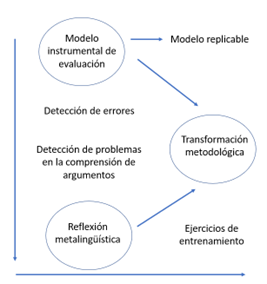
\includegraphics[width=\textwidth]{Fig2.png}
 \caption{Herramienta modelo de evaluación de textos argumentativos.}
 \label{fig2}
 \source{Elaboración propia}
\end{minipage}
\end{figure}

La aplicación del instrumento de evaluación y el posterior proceso de reflexión metalingüística en el aula a partir de los resultados del ejercicio valorativo suponen una transformación metodológica para el desarrollo de la comprensión de textos argumentativos, pues, en su complementación, se diagnostican los problemas y se resuelven desde el razonamiento y el ejercicio práctico. A su vez, el modelo instrumental que se ha diseñado en esta investigación se puede replicar adaptado a alumnos de distintas edades, niveles educativos y madurez discursiva, así como a textos argumentativos de mayor o menor complejidad. En este caso, se han introducido ocho conectores diversos para indagar patrones posibles de confusión que pudieran especificar problemas concretos en la comprensión de la cohesión argumentativa. En función de los destinatarios, la prueba debe adaptarse simplificando el texto: reduciendo su longitud total y la de cada oración, reduciendo el número de nociones argumentales y también la tipología de conectores. De hecho, la originalidad del procedimiento \emph{cloze}, como se ha expuesto, se debe a las pruebas DELE, que evalúan la comprensión lectora en los distintos niveles señalados en el Marco Común Europeo de Referencia para las Lenguas \cite{de2002marco}. Por tanto, la posibilidad de adaptar el instrumento a los distintos niveles de madurez lingüística en la lengua materna es perfectamente viable.

Los resultados de nuestra investigación muestran que:

\begin{enumerate}
    \item hay diferencias estadísticamente significativas en la proporción de aciertos (y, por tanto, dominio y comprensión) entre conectores y nociones argumentales; esto indica dónde hay que focalizar la intervención didáctica;
    \item existe una correspondencia casi exacta (excepto en un conector) entre la proporcionalidad de aciertos y su frecuencia de uso según el corpus CREA; esto significa que lo más frecuente en el uso acaba siendo más transparente semánticamente para los hablantes (acorde con los principios de la Teoría Natural, \textcite{dressler_morphonology_1985} y la semiótica discursiva, \textcite{kress2000semiotica}, por ejemplo);
    \item el análisis de errores muestra patrones de confusión entre ciertos conectores que son indicadores de los focos problemáticos en la comprensión; de este modo, las diferencias entre los conectores y los argumentos que ligan otorgando la cohesión al discurso deben tratarse mediante ejercicios de reflexión metalingüística contextualizados. En esta muestra ($N=125$), de manera especialmente significativa se confunden \emph{no obstante} (contraargumentación) y \emph{así pues} (consecuencia), \emph{más bien} (rectificación) y \emph{en definitiva} (recapitulación) y \emph{desde luego} (reforzamiento) y \emph{en cambio} (contraargumentación). La intervención didáctica se tendría que enfocar, con esta muestra de participantes, en estos conectores y argumentos.
\end{enumerate}

No se pueden elevar a categoría universal estos resultados, que pueden variar con un cambio de muestra. Pero el objetivo e interés de la investigación ha sido ver, por una parte, si el procedimiento \emph{cloze} para medir la comprensión lectora en ELE funcionaba también con la lengua materna y, por otra parte, comprobar qué información aportan los resultados más allá del déficit en la comprensión con el propósito de otorgar a la prueba el valor de modelo instrumental de evaluación. Como en otras investigaciones empíricas \cite{alvarez_dificultades_2017}, se ha probado que la dificultad de la comprensión en este tipo de textos está en el reconocimiento de argumentos, pero se llega a esta conclusión por las confusiones significativas en el uso de conectores (confusiones no bidireccionales de \emph{en cambio} y \emph{desde luego}). El modelo \emph{cloze} de evaluación de la comprensión de los textos argumentales apoyado en los conectores valora la cohesión discursiva global del texto y permite detectar dónde están los principales problemas de comprensión. A partir de los resultados de la aplicación de este modelo, avalado en el ámbito de evaluación de ELE, debería diseñarse la intervención didáctica motivando la conciencia metalingüística de los estudiantes y comprobando posteriormente, los progresos del proceso didáctico. Es decir, la prueba diagnostica dónde radica la comprensión deficiente y es a partir de la evaluación cuando deberá modelarse la intervención didáctica focalizada en los aspectos deficitarios. La evaluación forma parte del proceso formativo y el modelo instrumental de evaluación, como hemos visto en este caso, es clave para avanzar en el desarrollo de la comprensión textual.

\section{Financiación}
Investigación financiada dentro del proyecto I+D+i PID 2020-116110GB-100, concedido por el Ministerio de Ciencia e Innovación de España, con referencia MCIN/AEI/10.13039/501100011033.

\printbibliography\label{sec-bib}
% if the text is not in Portuguese, it might be necessary to use the code below instead to print the correct ABNT abbreviations [s.n.], [s.l.]
%\begin{portuguese}
%\printbibliography[title={Bibliography}]
%\end{portuguese}


%full list: conceptualization,datacuration,formalanalysis,funding,investigation,methodology,projadm,resources,software,supervision,validation,visualization,writing,review
\begin{contributors}[sec-contributors]
\authorcontribution{Rosa Ana Martín Vegas}[conceptualization,datacuration,formalanalysis,funding,investigation,methodology,projadm,validation,visualization,writing,review]
\authorcontribution{Marta Seseña Gómez}[conceptualization,datacuration,investigation,methodology,validation]
\end{contributors}

\end{document}

